\documentclass[12pt]{article}
\usepackage[brazil]{babel}
\usepackage{graphicx}
\usepackage{mathtools}
\usepackage{float} 
\usepackage{xcolor}


\usepackage{array}
\usepackage{booktabs}



% margenes
\usepackage[a4paper,left=2cm,right=2cm,top=1cm]{geometry}

%opening
\title{\textbf{Modelagem de Escoamentos Turbulentos. \\Lista de Exercícios No. 4}}

\author{Cristian Herledy López Lara}
\date{Julho 2025}

\begin{document}
	
\maketitle


\section*{Questão 1}

A relação proposta por Kolmogorov é usada em quase todos os modelos baseados no conceito de viscosidade turbulenta. Explique duas deficiências dessa proposta na previsão de escoamentos
turbulentos.\\


\textbf{\underline{Desenvolvimento}}

Partindo da equação da hipótese de Boussinesq, generalizada por Kolmogorov temos que 

\begin{equation}
	-\overline{u_i u_j} = \nu_t \left( \frac{\partial U_i}{\partial x_j} + \frac{\partial U_j}{\partial x_i} \right) - \frac{2}{3} k \delta_{ij}
\end{equation}


Para fazer a análise, começamos testando os índices numericamente e abrindo os termos da equação. Primeiro, quando $i=j=1$

\begin{equation}
	-\overline{u_1 u_1} = \nu_t \left( \frac{\partial U_1}{\partial x_1} + \frac{\partial U_1}{\partial x_1} \right) - \frac{2}{3} k \delta_{11} = 2\nu_t \left( \frac{\partial U_1}{\partial x_1}  \right) - \frac{2}{3} k
\end{equation}

Por exemplo, para o caso do escoamento plenamente desenvolvido $\frac{\partial U_1}{\partial x_1} = 0 $, que precisamente é o termo que 

\begin{equation}
	-\overline{u_1 u_1} = \frac{2}{3} k = \frac{2}{3}\left( \frac{\overline{uu} + \overline{vv} + \overline{ww}}{2}\right) 
\end{equation}

Pode-se observar que o modelo estã prevendo isotropía com o termo $\overline{uu} \sim  \overline{uu} + \overline{vv} + \overline{ww}$, o qual não é correto. Portanto, o modelo está subestimando $\overline{uu}$, falhando em capturar a anisotropia gerada pelo termo gradiente de velocidade.\\
Em sala de aula foi deducido que em escoamentos reales que \textbf{$uu\gg vv \sim ww$}, por tanto equação 3 não concorda com o que foi observado experimentalmente [2].\\


\section*{Questão 2}

Para a situação de escoamento turbulento da figura abaixo, identifique as razões pelas quais um modelo algébrico teria dificuldades em prever os níveis de turbulência corretamente na região de recirculação e na região do reatamento do escoamento.\\

\begin{figure}[H]
	\centering
	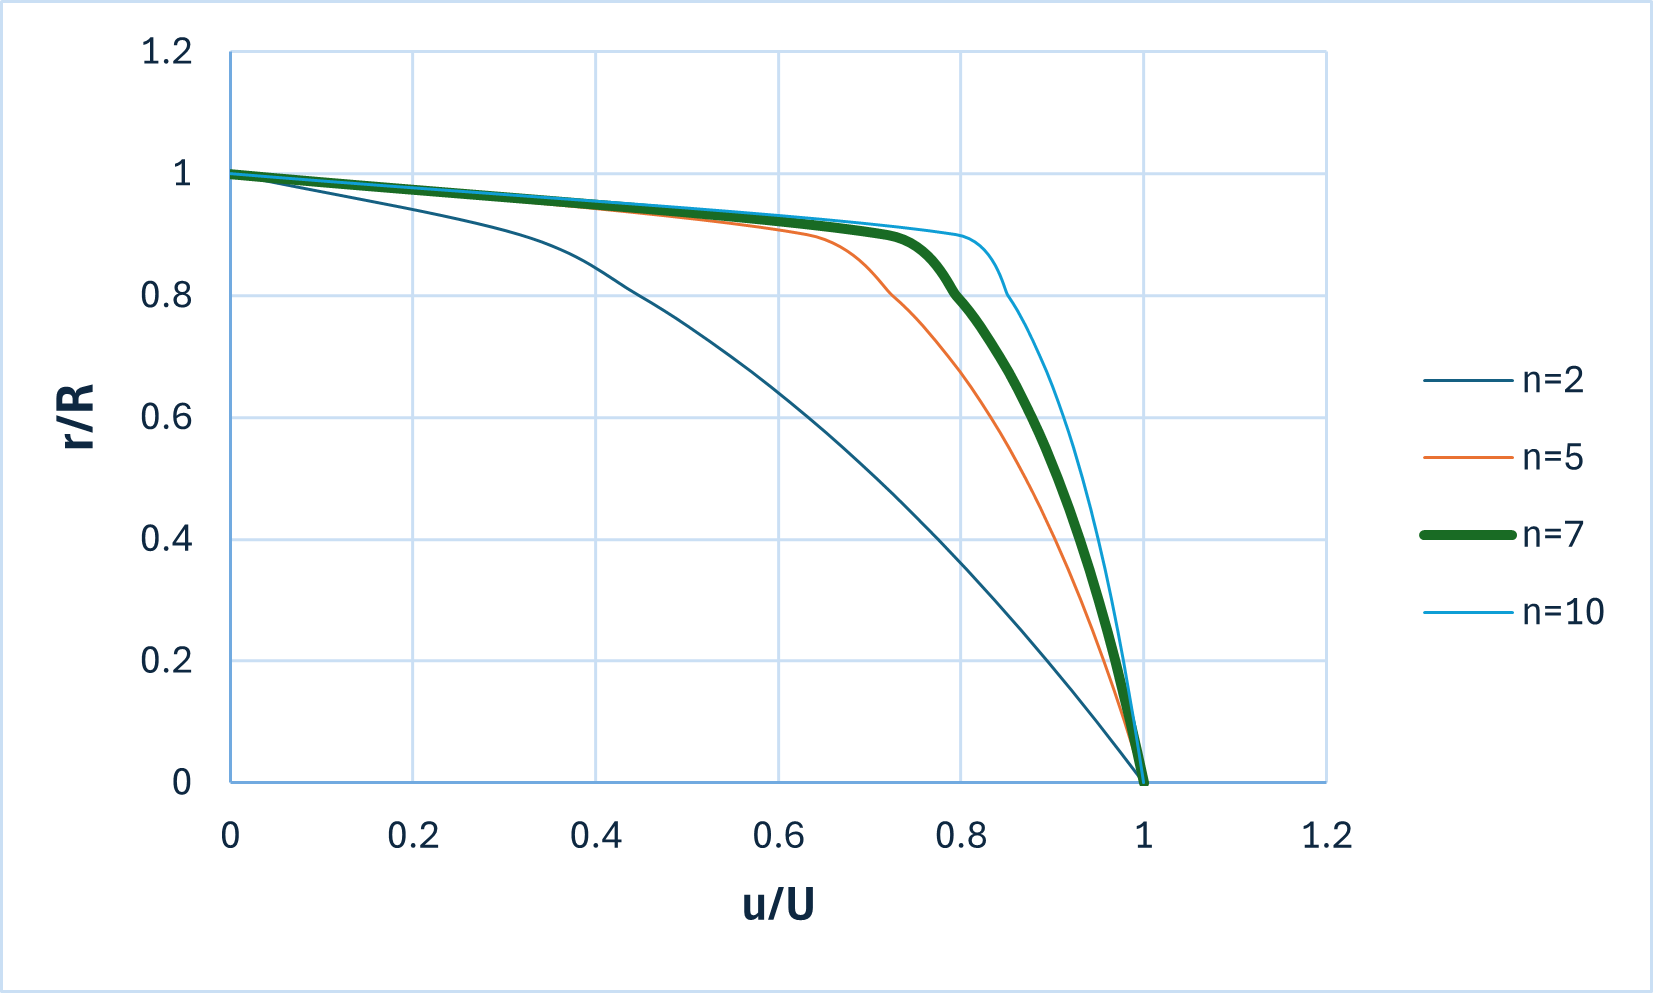
\includegraphics[width=.65\textwidth]{figures/1}
\end{figure}

\textbf{\underline{Desenvolvimento}}

A fugura mostra um escoamento que passa por um área de recirculação e de reatamento. Os modelos algebraicos sãó baseados no calculo da viscosidade turbulenta definida por a expressão

\begin{equation}
	\nu_t = lm^2\left\| \frac{\partial \overline{U}}{\partial y}\right\| 
\end{equation}.

Na área de recirculação, é esperado que la viscosidade turbulenta seja alta, devido as mudanças abruptas na direcão do escoamento e porque traz informações de memória da turbulência do contato com a parede anterior. Essas informações não están contidas no termo de $v_t$, que só depemde do gradiente de velocidade $\frac{\partial \overline{U}}{\partial y}$.

Na parte de reatamento o gradiente de velocidade pode se tornar negativo ou até nulo. Porem, a $\nu_t  \leq 0 $ o que está subestimando a turbulencia, e não é correto (os coeficientes de transporte de turbulencia não são desprezzíveis).


\section*{Questão 3}

O modelo RNG $k-\varepsilon$ é uma proposta para a previsão de escoamentos turbulentos. A principal diferença desse modelo em relação ao modelo $k-\varepsilon$ padrão é a equação da dissipação. Explique o efeito do termo R sobre o valor da viscosidade turbulenta em situações de
escoamentos com valores elevados de $S_{ij}$.\\

\textbf{\underline{Desenvolvimento}}

Da equação da dissipação

\begin{equation}
	U_j \frac{\partial \varepsilon}{\partial x_j} = 
	\frac{\partial}{\partial x_j} \left[ \left( \nu + \alpha \nu_t \right) \frac{\partial \varepsilon}{\partial x_j} \right]
	+ C_{\varepsilon 1} \frac{\varepsilon}{k} \nu_t S^2 
	- C_{\varepsilon 2} \frac{\varepsilon^2}{k} + R
\end{equation}
 Vamos analisar o efeito do termo R dado por 
\begin{equation}
	R = - \frac{C_\mu \, \eta^3 \left(1 - \eta / \eta_0 \right) \, \varepsilon^2}{1 + \beta \, \eta^3 \, k}
\end{equation}

Neste termo, a expressão $\eta = Sk/\varepsilon$ é contido e traze a informacão do balance entre a producão e a dissipacão da energ~ia transportada pela turbulencia. Neste termino, no numerador , emcontra se o tensor taxa de derformação dado pela expresão

\begin{equation}
	S_{ij} = \frac{1}{2} \left( \frac{\partial U_i}{\partial x_j} + \frac{\partial U_j}{\partial x_i} \right)
\end{equation}

Agora, considerando que
\begin{equation}
	R \sim  \frac{\left(1 - \eta / \eta_0 \right) }{1 +  \eta^3}
\end{equation}

Então para escoamentos com altas taxas de deformação $S_{ij}$, $\frac{\eta}{\eta_0} > 1$ e porem $R<0$, o que reduz a taxa de dissipaçao.

A viscosidade turbulenta é dada pela expressão

\begin{equation}
	\nu_t = C_\mu \frac{k^2}{\varepsilon}
\end{equation}

Portanto, ao reduzir o valor de $\varepsilon$, tem como efeito um aumento da viscosidade turbulenta. Permitindo aos modelos baseados no calculo de  $\nu_t$ capturar melhor os efeitos em escoamentos com grandes gradientes de velocidade.


\section*{Questão 4}

Indique a vantagem de uma característica particular dos modelos de turbulência SST e Realizável.\\

\textbf{\underline{Desenvolvimento}}

Os dois modelos presentam uma vantagem comum: ajustam seus parâmetros ddependendo das condições locais do escoamento

\begin{itemize}
	\item No modelo SST, isso ocorre por meio da função $F_1$ [1] ajustando a transição entre modelos locamente dentro da camada limite.
	\item No modelo realizável, o parâmetro $C_\mu$ varia garantindo tensões coerentes com as mudanças da turbulência do escoamento.
\end{itemize}


\section*{Questão 5}

Explique a necessidade do uso do perfil logarítmico de velocidade na prescrição da condição de contorno de paredes sólidas em modelos de turbulência para altos números de Reynolds.\\

\textbf{\underline{Desenvolvimento}}

\begin{equation}
	U^+ = \frac{1}{\kappa} \ln(E \, y^+)
\end{equation}


O uso do perfil logarítmico é necessário na prescrição da condição de contorno de paredes sólidas em modelos de turbulência com altos números de Reynolds, pois modelos de turbulencia como $k-\varepsilon$ ou $k-\omega$, não resolvem adequadamente os gradientes de velocidade proximo a parede. \\
Em escoamentos con alta velocidade (alto número de Reynolds), a camada límite é bastante mais fina. Assim, estos modelos requerem uma discretização espacial muito pequena para capturar os efeitos do transporte difusivo molecular, o que resulta computacionalmente muito caro.

O perfil logarítmico fornece uma aproximação adequada para o escoamento  na camada límite, garantindo uma transição suave entre a parede e o interior do escoamento.

Além disso, o perfil logarítimico fornece o cálculo certo da condiçao de contorno de tensão cisalhante prescrita  muito próximo a superficie onde $y^+ <11$, que logo é acoplada com o escoamento dominado por $\overline{u_i u_j}$.

\section*{Questão 6}

Considere um escoamento turbulento incompressível sobre uma superfície côncava como ilustrada abaixo.\\
\begin{figure}[H]
	\centering
	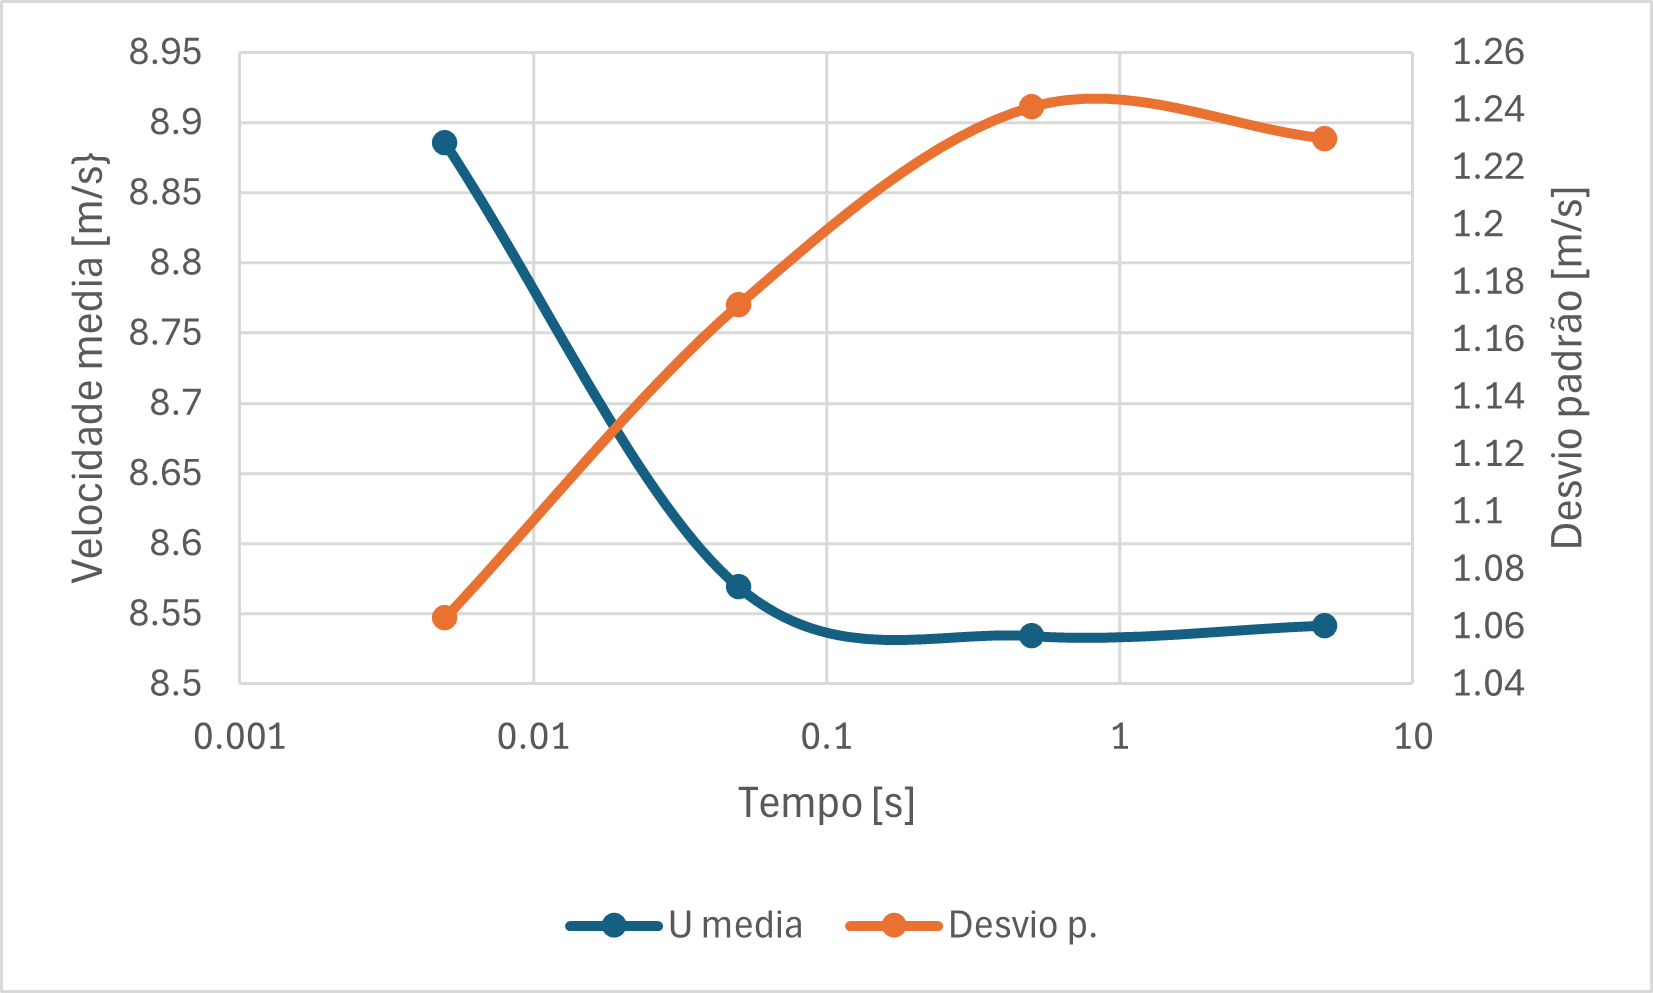
\includegraphics[width=.65\textwidth]{figures/2}
\end{figure}


A partir da análise do termo de produção para as tensões de Reynolds,  demonstre que mesmo uma curvatura suave da superfície pode afetar de forma significativa a tensão cisalhante junto à parede.\\

\textbf{\underline{Desenvolvimento}}

Partindo da equaçao do termo de produçao temos que 
\begin{equation}
	P_{ij} \equiv - \overline{u_i u_k} \frac{\partial U_j}{\partial x_k}
	- \overline{u_j u_k} \frac{\partial U_i}{\partial x_k}
\end{equation}

 	

Calculando para $i=1, j=2$, para o analise do efeito em $\overline{uv}$

\begin{equation}
	P_{12} \equiv - \overline{u_1 u_k} \frac{\partial U_2}{\partial x_k}
	- \overline{u_2 u_k} \frac{\partial U_1}{\partial x_k}
\end{equation}

Abrindo para k
\begin{equation}
	P_{12} \equiv - \overline{u_1 u_1} \frac{\partial U_2}{\partial x_1}
	- \overline{u_2 u_1} \frac{\partial U_1}{\partial x_1} - \overline{u_1 u_2} \frac{\partial U_2}{\partial x_2}
	- \overline{u_2 u_2} \frac{\partial U_1}{\partial x_2}
\end{equation}

Então

\begin{equation}
	P_{12} \equiv - \overline{uu} \frac{\partial V}{\partial x}
	- \overline{vu} \frac{\partial U}{\partial x} - \overline{uv} \frac{\partial V}{\partial y}
	- \overline{vv} \frac{\partial U}{\partial y}
\end{equation}

\begin{equation}
	P_{12} \equiv - \overline{uu} \frac{\partial V}{\partial x}
	- \overline{vv} \frac{\partial U}{\partial y} - \left( \overline{vu} \frac{\partial U}{\partial x} - \overline{uv} \frac{\partial V}{\partial y}\right) 
\end{equation}

Os termos dentro dos parênteses são iguais a zero pela equação da continuidade, ficando

\begin{equation}
	P_{12} \equiv - \overline{uu} \frac{\partial V}{\partial x}
	- \overline{vv} \frac{\partial U}{\partial y}
\end{equation}

Obtem-se que, mesmo quando $\frac{\partial V}{\partial x}\ll \frac{\partial U}{\partial y}$, a magnitude da tensão normal $uu \gg vv$ junto a parede, faz que o primeiro termo tenha mais peso na produçao de $\overline{uv}$.

\section*{Questão 7}

Rotta (1951) propôs a seguinte forma modelada para o termo de redistribuição de energia em escoamentos onde as taxas de deformação do escoamento são nulas. Explique como esse termo funciona em escoamentos com anisotropia.\\

\begin{equation}
	\phi_{ij,1} = - c_1 \frac{\varepsilon}{k} \left( \overline{u_i u_j} - \frac{2}{3} k \delta_{ij} \right)
\end{equation}


\textbf{\underline{Desenvolvimento}}

O termo mostrado (termo rápido) actua na redistribução de energ~ia turbulenta. Em regiões de alta anisotropía, perto da parede poe exemplo, as magnitudes de los termos da tensão normal de Reynolds tem valores diferentes [2]


\begin{figure}[H]
	\centering
	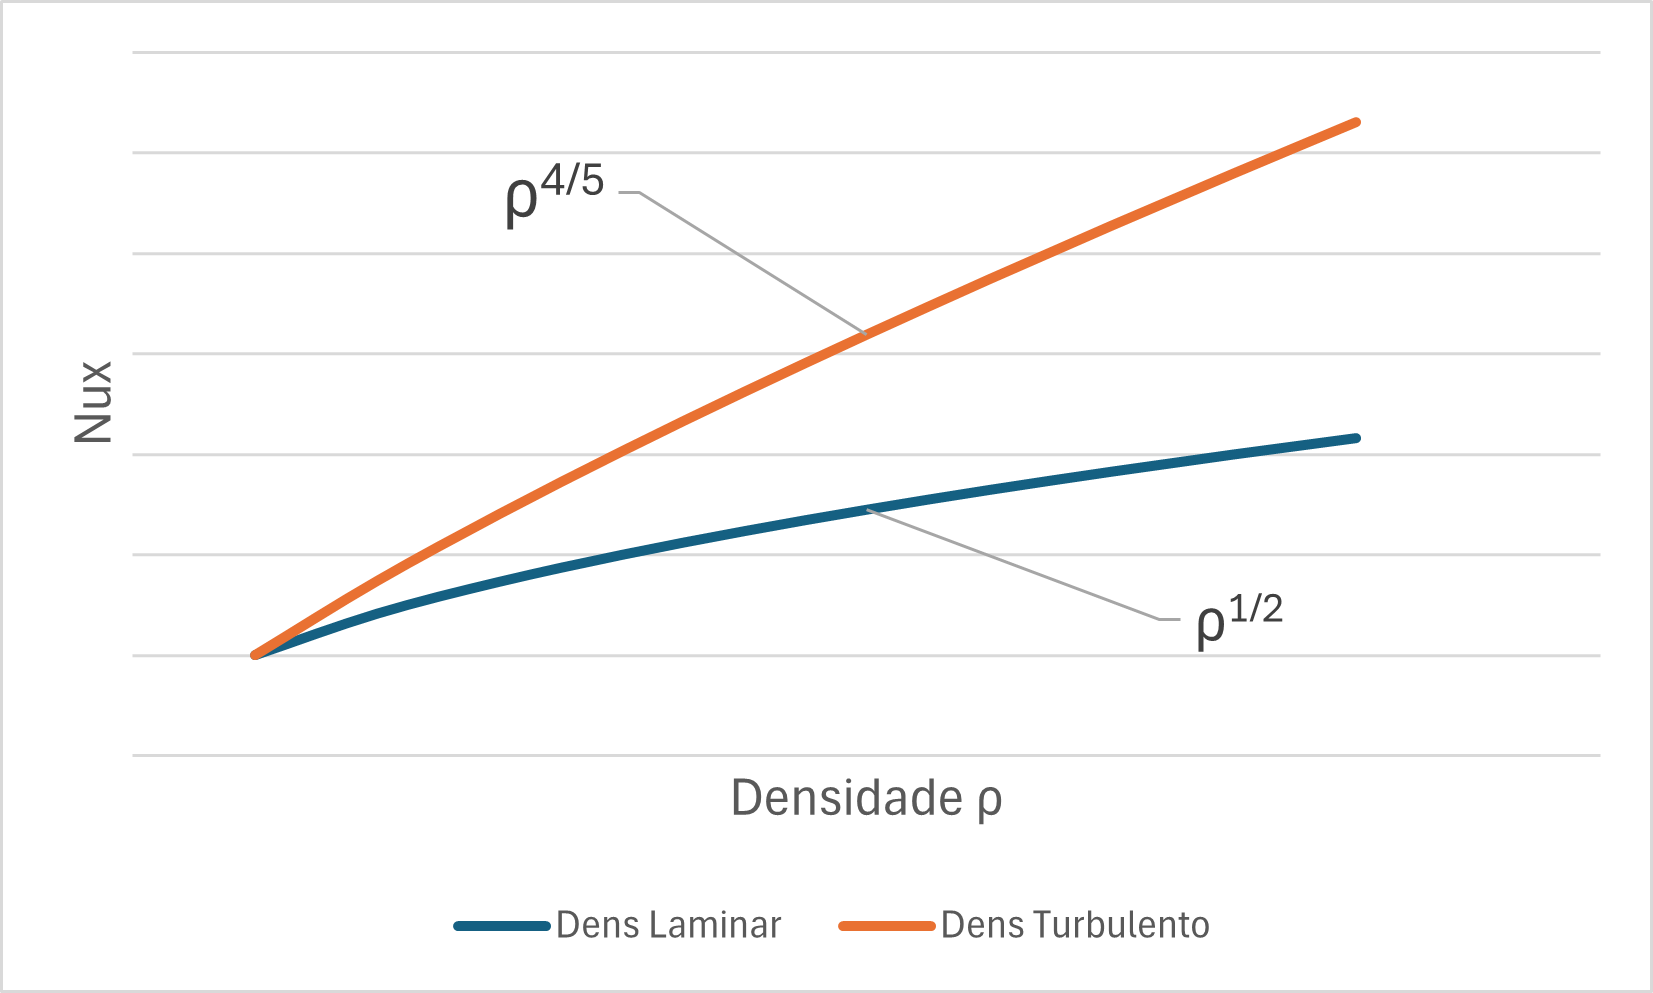
\includegraphics[width=.65\textwidth]{figures/3}
\end{figure}

Portanto, no exemplo da tabela, como $uu\gg vv \sim ww$, podemos analisar o termo para i=j


\begin{equation}
	\phi_{11,1} = - c_1 \frac{\varepsilon}{k} \left( \overline{u_1 u_1} - \frac{2}{3} k \delta_{11} \right)
\end{equation}


\begin{equation}
	\phi_{22,1} = - c_1 \frac{\varepsilon}{k} \left( \overline{u_2 u_2} - \frac{2}{3} k \delta_{22} \right)
\end{equation}

\begin{equation}
	\phi_{33,1} = - c_1 \frac{\varepsilon}{k} \left( \overline{u_3 u_3} - \frac{2}{3} k \delta_{33} \right)
\end{equation}

Pode-se notar que, olhando os valores da tabela, que $\phi_{11,1} > 0$ e $\phi_{22,1}, \phi_{33,1}  < 0$. Porem, $\overline{uu}$ vai diminuir, mesmo que $\overline{vv}$ e $\overline{ww}$ aumentan. Ou seja, o termo de Rotta preve a redistribução da energia turbulenta levando a un escoamento mais isotrópico.

\section*{Questão 8}

Vimos que a equação de $\varepsilon$ é uma das principais fontes de erro nos modelos de turbulencia. No caso do modelo de transporte de $\overline{u_i u_j}$, como podemos identificar se eventuais falhas na previsão de $\overline{u_i u_j}$ provém de erros da equação de $\varepsilon$ ou das formas modeladas dos termos de redistribuição e difusão\\


\textbf{\underline{Desenvolvimento}}
Podem se revisar varios pontos no transporte de $\overline{u_i u_j}$ [2]

\begin{itemize}
	\item Da questão anterior, o termo de redistribução $\phi_{ij,1}$ tem um efeito significativo no cãlculo de $\overline{u_i u_j}$. Se as propocões de $\overline{u_i u_j}$ não comcordan com a física do problema, a anisotropía não será bem resuelta e por tanto a energía turbulenta será errada. Pode ser validado com seguimento da anisotropía en regiões donde podam ser esperadas, como proximo das paredes.
	\item O termo de transporte difusivo podem producir oscilaciones não físicas em áreas de altos gradientes. Pode ser pode ser detectado com flutuações anormais de $\overline{u_i u_j}$
	\item O termo mais relevante ~e o termo de dissipaçao $\varepsilon$. Da equação (9) pode ser visto que $\nu \sim \varepsilon^{-1}$. Porem, erros no calculo dos valores de $\overline{u_i u_j}$, podem vir de estimaciones erradas da trasnferencia de energía das grandes as pequenas escalas.  
\end{itemize}


\begin{thebibliography}{999}
	
	
	\bibitem{Deschamps}
	Cesar Deschamps,
	Modelos de viscosidade turbulenta Cap 4.
	UFSC Florianopolis, SC,
	Notas de aula,
	2025.
	
	\bibitem{Deschamps}
	Cesar Deschamps,
	Modelos dr trasnporte para as tensões de Reynolds. Cap 5.
	UFSC Florianopolis, SC,
	Notas de aula,
	2025.
		
	
\end{thebibliography}


\end{document}





